\documentclass{article}
\usepackage[utf8]{inputenc}
\usepackage{hyperref}
\usepackage{graphicx}
\usepackage{float}
\usepackage[skip=10pt, indent=20pt]{parskip}
\graphicspath{{./figures/}{./lessons/02-hello-world/assets/docs/figures/}}

\title{Lesson 2 - Hello World}
\author{Bryan A. \textit{CrazyUncleBurton} Thompson \\ \textit{bryan@batee.com}}
\date{March 17, 2026}

\begin{document}

\maketitle

\section*{Overview}
This lesson will show you how to compile and upload a basic "Hello World" 
program to a microcontroller.
\vspace{3mm}

\section*{Theory}
This is our first program, and we’re learning a lot of things all at once. 
We make the circuit as easy as possible by using a pre-built module which 
only connects one way to the microcontroller.
\vspace{3mm}

\section*{Hardware Required}
The following hardware is needed for this lesson:

1-M5Stack Tab5 Microcontroller Development Board

1-M5Stack Dual LED Module

1-4 wire M5Stack sensor cable 

1-USB cable to connect the Tab5 USB-C port to your PC
\newpage

\section*{Objectives}
\begin{itemize}
  \item Familiarity with the Tab5 development board
  \item Familiarity with VS Code IDE
  \item Create our first electric circuit
  \item Compile our first program
  \item Upload a basic “Hello World” program to the development board
  \item Test the program
\end{itemize}
\newpage


\section*{The M5Stack Tab5 Microcontroller Development Board}

\vspace{3mm}
\begin{figure}[H]
    \centering
    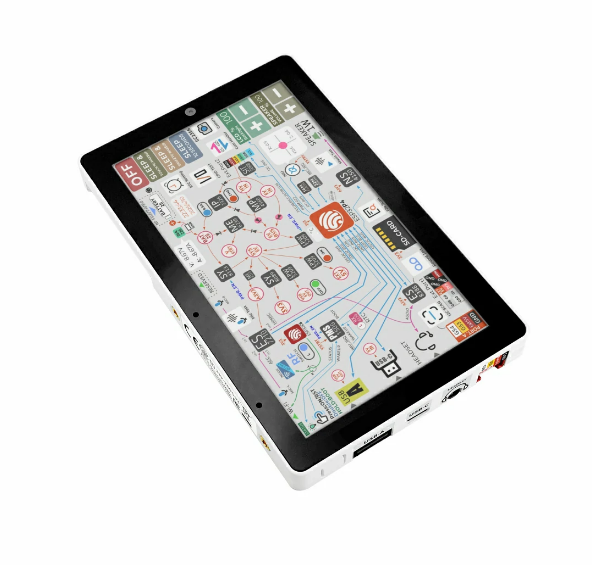
\includegraphics[width = .8\linewidth]{m5stack-front.png}
    \caption{The M5Stack Tab5 Development Board}
\end{figure}

M5Stack.com is owned by Espressif, the manufacturer of the microcontroller 
inside the Tab5.  We chose it for the ultimate in support by the manufacturer.
The M5Stack Tab5 microcontroller development board has an ESP32-P4 
microcontroller with three cores, two of which run at 360MHz.  

It has an ESP32-C6 Communications IC with 
support for 2.4 GHz Wi-Fi 6, Bluetooth 5 (LE), Zigbee 3.0, and Thread 1.3.  
It has a 5” LCD touchscreen, camera, microSD slot, Audio Inputs and Outputs, 
Microphones, a Real Time Clock, a 6-axis accelerometer/gyro sensor, and many 
ways to connect to external circuits!
\newpage

The manufacturers' datasheet for the Tab5 is located here.  You can find 
information like schematics, external hardware connections and more: \\ 
\url{https://docs.m5stack.com/en/core/Tab5}

M5Stack provides a super-rich development ecosystem, including sensors, modules
and accessories:  \\
\url{https://shop.m5stack.com/collections/unit }



\vspace{3mm}

\begin{figure}[H]
    \centering
    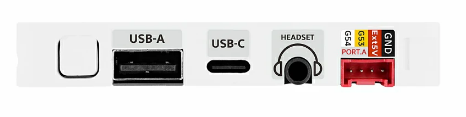
\includegraphics[width = .8\linewidth]{m5stack-bottom.png}
    \caption{Tab5 Bottom Side}
\end{figure}
\vspace{3mm}
 
\subsection*{Powering the Tab5 On and Off}
\begin{enumerate}
    \item We can supply power to the Tab5 through its USB-C port.  Connect
    the Tab5 USB-C port to your computer with a USB cable.
    \item The white “U” shaped button on the left is the On/Reset/Off button.  
    \item Press the button once to turn on the screen.  You should see the 
    factory firmware running on the controller.  It shows some useful data 
    about the hardware and some live data on the LCD:
    \vspace{3mm}
    \begin{figure}[H]
        \centering
        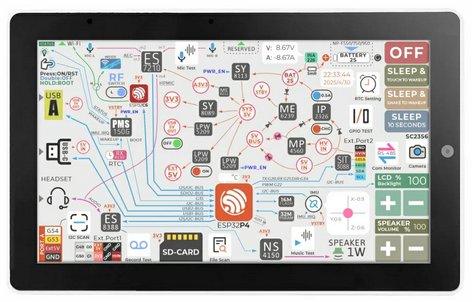
\includegraphics[width = .8\linewidth]{tab5-on.png}
        \caption{Tab5 Running Factory Firmware}
    \end{figure}
    \vspace{3mm}
    \item Press and release the power button once.  Note that the unit powers 
    off and back on (we call this a reset).
    \item Double press and release the power button to turn the controller off.
    
\end{enumerate}
\newpage

\section*{The PORT.A Input / Output Connector}
\vspace{3mm}
\begin{figure}[H]
    \centering
    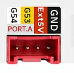
\includegraphics[width = .2\linewidth]{m5stack-porta-connector.png}
    \caption{The PORT.A Input/Output Connector}
\end{figure}
\vspace{3mm}
PORT.A can be configured for GPIO digital I/O and serial communication via UART
or I2C. This enables quick, plug-and-play connectivity for sensors and actuators.

This is a 4-pin HY2.0-4P Grove connector.  It's similar to a 4 pin JST PH connector.

\vspace{3mm}
\begin{figure}[H]
    \centering
    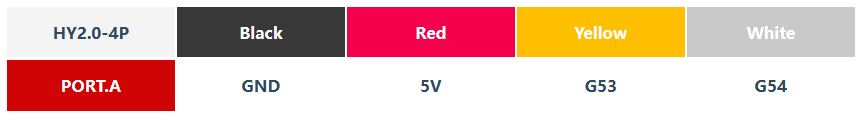
\includegraphics[width = .8\linewidth]{porta-table.png}
    \caption{PORT.A Pins and their Functions}
\end{figure}
\vspace{3mm}

There are four pins on the PORT.A connector:

\begin{itemize}
    \item Black - GND: Ground is the common reference terminal against which 
    other outputs are measured.
    \item Red - 5V: This is a 5V reference / power supply from the port, 
    intended to power any sensors or actuators.  \textit{Why is it 5V when we're 
    working in a 3.3V ecosystem?}  My guess is to let us power and communicate 
    with 5V sensors as well as 3.3V ones.
    \item Yellow - G53 and White - G54:
    The Yellow wire is connected to pin G53 on the microcontroller.
    The White wire is connected to pin G54 on the microcontroller.  
    These wires can be turned on and off by the program. When on, the wire will be 
    +3.3V with respect to ground.  When off, it will be 0V.
\end{itemize}
\newpage
\vspace{3mm}

\section*{The Dual LED Module}
In embedded electronics programming, our version of the Hello World program
is called Blinky (or just "blink"): we simply try to make an LED blink because that
is the simplest way to prove that the microcontroller is loading and executing our
programs.

Unfortunately, there's not a blinkable LED built into our Tab5 Dev board
(a huge oversight on the part of M5Stack).  But CrazyUncleBurton didn't let that stop
him - he bought some prototype modules and built his own!
\vspace{3mm}
\begin{figure}[H]
    \centering
    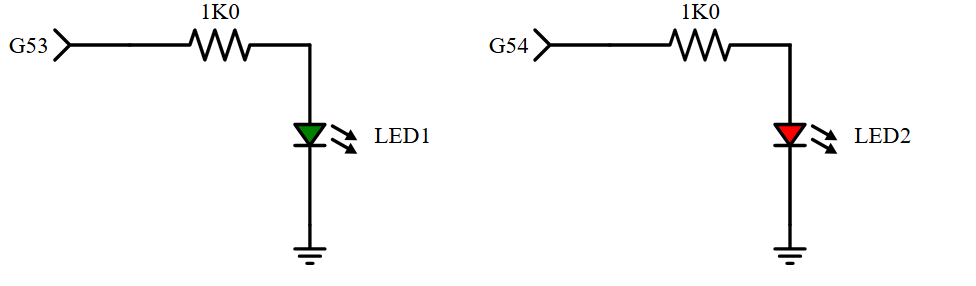
\includegraphics[width = .4\linewidth]{dual-led-module.png}
    \caption{The Dual LED Module}
\end{figure}
\vspace{3mm}
There are two independent circuits inside the Dual LED Module.  Well, they share 
the ground terminal of the port, but that's it.
\vspace{3mm}
\begin{figure}[H]
    \centering
    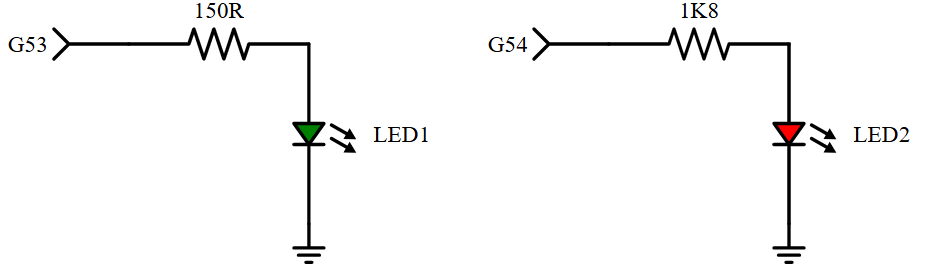
\includegraphics[width = .8\linewidth]{dual-led-circuit.png}
    \caption{The Dual LED Module Schematic}
\end{figure}
\vspace{3mm}

The green LED is connected to GPIO pin G53.  When GPIO pin G53 is set to a 
logic high, the ESP32 outputs 3.3V to pin G53 and the green LED lights. When
pin G53 is set to a logic low, the ESP32 outputs 0V to pin G53 and the 
green LED turns off. The red LED works in exactly the same way, except that its
signal is passed through GPIO pin G54. 

In the green LED's circuit, a 150$\Omega$ (ohms) resistor limits current to about
8.6mA.  In the red LED's circuit, a 1.8K$\Omega$ resistor limits current to about
0.72mA. Limiting the current is necessary to protect the microcontroller and the LED.  
\vspace{3mm}

\section*{Connections}

\begin{enumerate}
    \item To connect the Dual LED module to the Tab5 dev board, use the 4 wire
    cable supplied with the module. Plug one end into the Dual LED module and
    the other into the Tab5 dev board.  
    \vspace{3mm}

    \begin{figure}[H]
        \centering
        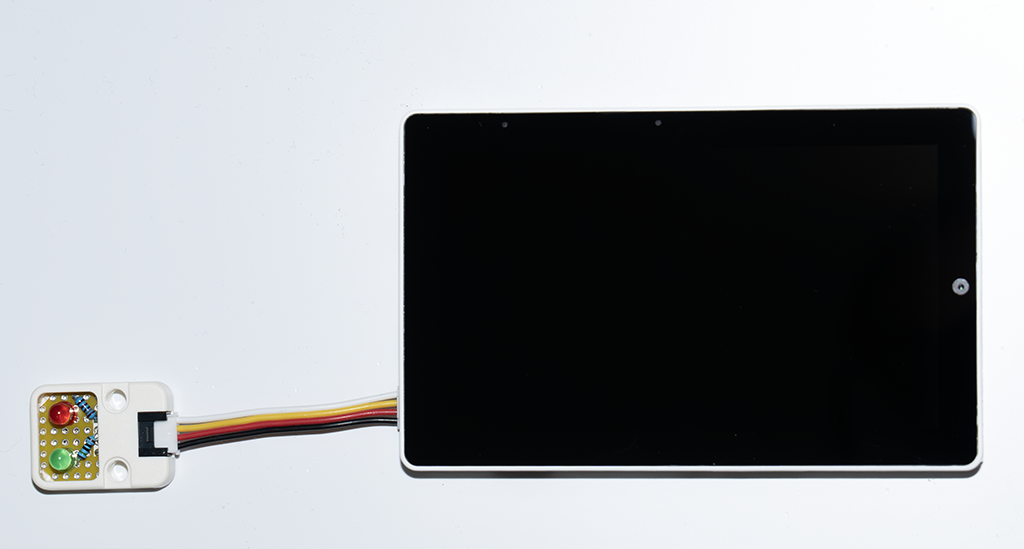
\includegraphics[width = 1\linewidth]{led-module-connected.png}
        \caption{Dual LED Module Connected to Tab5}
    \end{figure}
    \vspace{3mm}
    \item Connect the Tab5 to the computer via the USB-C port.
\end{enumerate}
\newpage

\section*{The Program}

Our program is located in the folder \path{02-hello-world/code/2-blink}:

\vspace{3mm}
\begin{figure}[H]
    \centering
    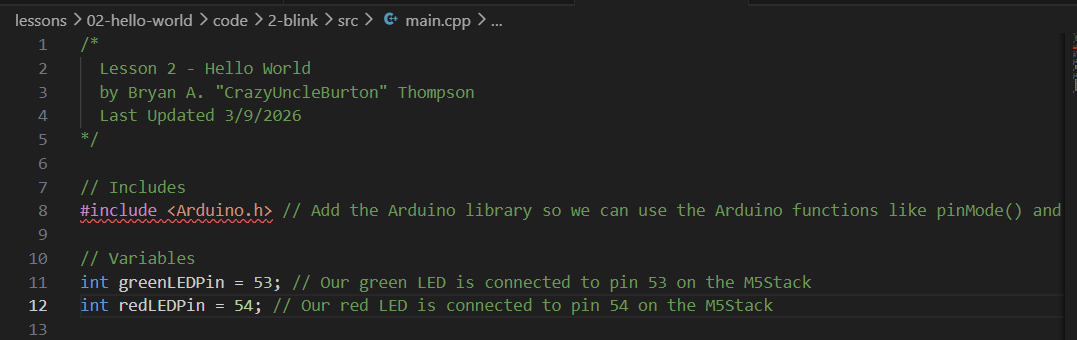
\includegraphics[width = 1\linewidth]{program-1.png}
    \caption{Hello World Program - Part 1}
\end{figure}
\vspace{3mm}

Lines 1-5 are a block comment that lets the user know who to yell at when this 
doesn't work.
\vspace{3mm}

Line 8 is an "include" directive.  This tells the C++ compiler's linker to link a
"header file" named "Arduino.h" to the top of this C++ source code file.
This header file contains code from Arduino that we can borrow to use in our own
programs.  Specifically, we want the \textbf{pinMode()} 
command, which lets us declare the GPIO pin to be an output, and the 
\textbf{digitalWrite()} command, which will turn GPIO pins on and off.

Lines 11 and 12 initialize global variables of the integer type.  The variables are 
named \textbf{greenLEDPin}, which we set to 53 (for GPIO pin 53), and \textbf{redLEDPin},
which we set to 54 (for GPIO pin 54).  

\begin{figure}[H]
    \centering
    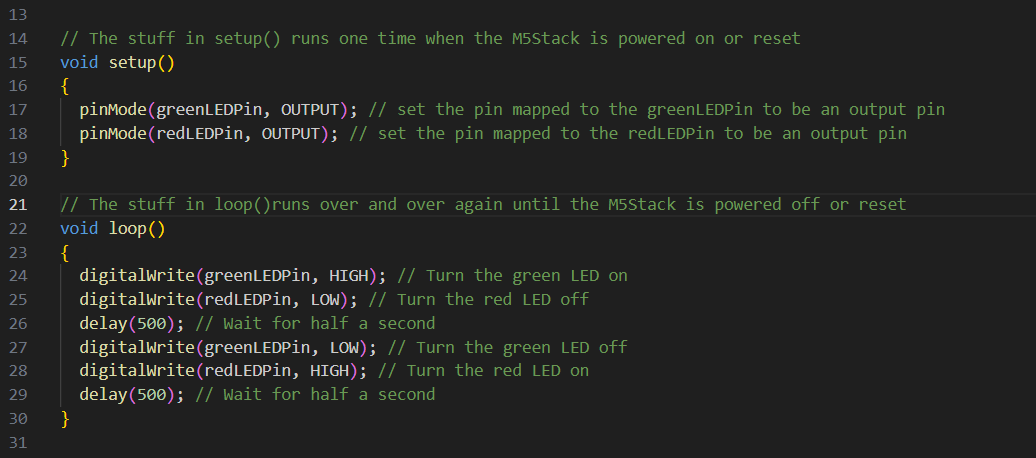
\includegraphics[width = 1\linewidth]{program-2.png}
    \caption{Hello World Program - Part 2}
\end{figure}
\vspace{3mm}

On lines 15 and 22, you will see two functions: \textbf{setup()} and \textbf{loop()}.

In standard Arduino programs, you prepare or \textit{initialize} ("init") the
microcontroller and any additional components with code in the setup() function.
This function is run \textit{once} whenever the microcontroller is powered on or reset.

In lines 17 and 18, we set GPIO pins 53 and 54 to be digital outputs by calling
the pinMode() function on variables \textbf{greenLEDPin} and \textbf{redLEDPin}.

Digital output pins can output two levels:  
\begin{itemize}
    \item Digital logic level 1, or "high," which makes that output pin +3.3V
    \item Digital logic level 0, or "low," which makes that output pin 0V.
\end{itemize}

Once the setup() function finishes, it hands control over to the loop() function.

The loop() function contains all of the code that we would consider "the program."
When the function ends, it starts over and runs all of the same code again,
just like the name suggests.

\vspace{3mm}
\textbf{Important Point:} Most embedded programs are required to loop infinitely!
Otherwise, once the program is finished, the microcontroller will run out of
instructions and do absolutely nothing until the device is reset.
\vspace{3mm}

Line 24 sets \textbf{greenLEDPin} to \textbf{High}, which turns the green LED on,
and line 25 sets the \textbf{redLEDPin} to \textbf{Low}, which turns the red LED off.

Line 26 is a delay.  It waits 500 milliseconds (one half-second) before proceeding.

Lines 27 and 28 do the reverse of lines 24 and 25. Line 27 sets \textbf{greenLEDPin}
to \textbf{Low}, which turns the green LED off, and line 28 sets the \textbf{redLEDPin}
to \textbf{High}, which turns the red LED on.

Lines 26 is a delay.  It waits 500 milliseconds (one-half second) before 
proceding.
\newpage

\section*{Compiling and Uploading the Program}

When the microcontroller is powered on, it first runs its \textit{bootloader} code,
which in our case will help VS Code upload programs to the microcontroller.
The bootloader is preloaded on the Tab5 at the factory, and remains in place when programs
are uploaded to the microcontroller.

When a program is uploaded to the Tab5, it is stored in FLASH memory on the
microcontroller.  FLASH memory is \textit{persistent} - it retains the program even after
it loses power. It is memory though, not like a hard drive, which is a disk.

\begin{enumerate}
    \item See the upload port icon at the bottom of the screen. Ensure the upload 
    port is set to \textbf{Auto}. 
    \vspace{3mm}
    \begin{figure}[H]
        \centering
        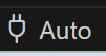
\includegraphics[width = .25\linewidth]{upload-port.png}
        \caption{PlatformIO: Upload Port}
    \end{figure}
    \vspace{3mm}
 
    \item Make sure the \textbf{Switch PlatformIO Project Environment} icon 
    at the bottom of the screen is set to \textbf{2-blink}.  This will ensure
    that we compile the correct code (there are many individual programs in
    the Microcontroller Training folder):
    \vspace{3mm}
    \begin{figure}[H]
        \centering
        
\includegraphics[width = .5\linewidth]{switch-platformio-project-environment.png}
        \caption{Switch PlatformIO Project Environment}
    \end{figure}
    \vspace{3mm}
       \item To compile the program and upload it to the microcontroller, click 
    on the \textbf{PlatformIO: Build} icon at the bottom of the screen:
    \vspace{3mm}
    \begin{figure}[H]
        \centering
        
\includegraphics[width = .25\linewidth]{upload.png}
        \caption{PlatformIO: Upload}
    \end{figure}
    \vspace{3mm}

    \item The results of the compile and upload process are presented in the 
    terminal window at the bottom of the screen:
    \vspace{3mm}
    \begin{figure}[H]
        \centering
        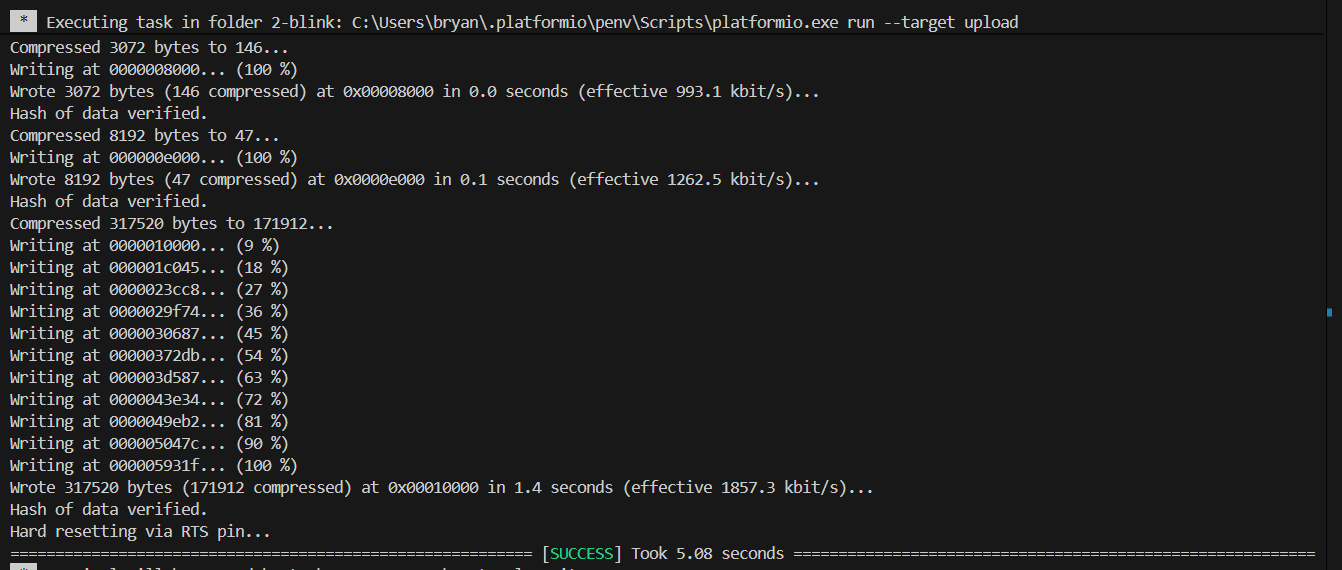
\includegraphics[width = 1\linewidth]{compiled.png}
        \caption{Program Compiled and Uploaded Successfully}
    \end{figure}
    \vspace{3mm}

\end{enumerate}
\vspace{3mm}

When the program uploads and the microcontroller reboots, we should see the red 
and green LEDs alternating on and off every half-second, or 500 milliseconds.

If you have a battery for your Tab5, you can disconnect it from the computer and
reset. Since the program is stored in FLASH memory, it should work just as before!
\vspace{3mm}

\section*{Modifying the Program}

Change the delay(500) lines to read delay(100).  Then build and upload again.
You should see the LEDs blink much faster!

\textbf{Exercise: on-on $\rightarrow$ off-off program}

Using only the \textbf{digitalWrite()} and \textbf{delay()} functions, write a program
that does the following:

\centering
Green ON $\rightarrow$ Red ON $\rightarrow$ Green OFF $\rightarrow$ Red OFF

Use delays so that the LEDs do not toggle on and off at the same time.
\newpage

\section*{Conclusions}
This completes the Hello World lesson.  We learned these concepts:

\begin{itemize}
    \item How to connect a circuit to the microcontroller
    \item How to configure pins on the microcontroller as digital outputs
    \item How to turn the pin on and off programatically
    \item How to compile and upload a program to the microcontroller
    \item How to make the microcontroller wait for a specific period of time
\end{itemize}
\vspace{3mm}

In the next lesson, we will introduce the LCD screen.

\end{document}
